\section{Auswertung}
\label{sec:Auswertung}

\subsection{Vorbereitung}

Die Größen Ordnungszahl $Z$, Literaturwert der
K-Kante $E_\text{K}^\text{Lit}$, der zugehörige Glanzwinkel 
$\Theta_\text{glanz}^\text{Lit}$ und die Abschirmkonstante 
$\sigma_\text{K}$ verschiedener Elemente in Tabelle 
\ref{tab:literatur} aufgelistet.

\begin{table}
  \centering
  \caption{Literaturwerte und daraus errechnete Größen verschiedener Elemente}
  \label{tab:literatur}
  \sisetup{table-format=2.1}
  \begin{tabular}{c c c c c}
  \toprule
  $ $ & $Z$ & $E_\text{K}^\text{Lit} \,/\, \si{\kilo\eV}$
  & $\Theta_\text{glanz}^\text{Lit} \,/\, \si{\degree}$ & 
  $\sigma_\text{k}$\\
  \midrule 
  13.623 & 11.052 & 9.758 & 7.325 & 6.377 &  \\
  13.700 & 11.021 & 9.723 & 7.288 & 6.419 &  \\
  13.657 & 10.964 & 9.737 & 7.252 & 6.417 &  \\
  13.614 & 11.038 & 9.687 & 7.259 & 6.393 &  \\
  13.699 & 10.952 & 9.681 & 7.245 & 6.379 &  \\
  \bottomrule
  \end{tabular}
  \end{table}




\subsection{Überprüfung der Bragg Bedingung}

Nach der Braggbedingung ist zu erwarten, dass das gemessene Intensitätsmaximum
für den errechneten Glanzwinkel auftritt. 

Die Berechnung erfolgt über die Umstellung der Gleichung \eqref{eqn:Bragg} zum Glanzwinkel
hin und durch Einsetzen des Ausdrucks $\lambda = \frac{h \cdot c}{E}$ zu 

\begin{equation}
  \Theta_\text{glanz} = \text{arcsin}\left(\frac{h \cdot c}{E \cdot 2d}\right)
\end{equation}

Mit einer Gitterkonstanten $d_\text{LiF} = \SI{201.4}{\pico\meter}$ und 




\begin{figure}
  \centering
  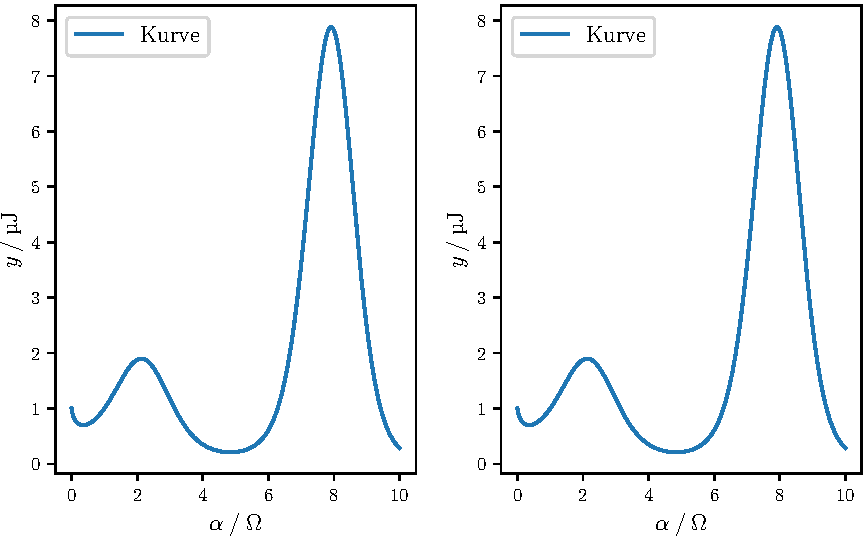
\includegraphics{plot.pdf}
  \caption{Plot.}
  \label{fig:plot}
\end{figure}
